\documentclass[margin=2cm]{standalone}

\usepackage{tikz}
\usetikzlibrary{shapes,% for the rectangle
                chains,% provides the chains
                scopes}% allows to replace \begin{scope} \end{scope} with {}

\begin{document}
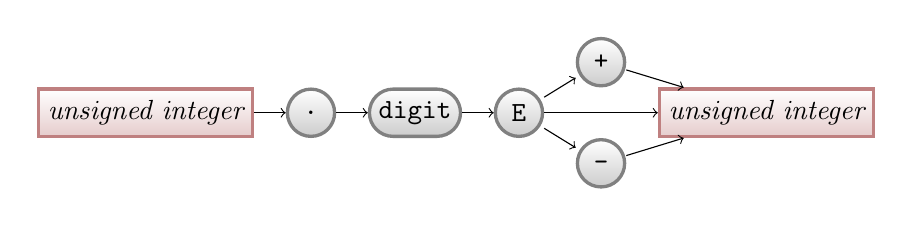
\begin{tikzpicture}[
  nonterminal/.style={
    rectangle, 
    minimum size=6mm, 
    very thick, 
    draw=red!50!black!50, 
    top color=white, % a shading that is white at the top...
    bottom color=red!50!black!20, % and something else at the bottom
    font=\itshape
  },
  terminal/.style={
    rectangle,minimum size=6mm,rounded corners=3mm,
    very thick,draw=black!50,
    top color=white,bottom color=black!20,
    font=\ttfamily
  },
  every on chain/.style={join}, every join/.style={->}
]

\matrix[column sep=4mm] {
  % First row:
  & & & & \node (plus) [terminal] {+};&\\
  % Second row:
  \node (ui1)   [nonterminal] {unsigned integer};&
  \node (dot)   [terminal]    {.};               &
  \node (digit) [terminal]    {digit};           &
  \node (e)     [terminal]    {E};               &
  & % space in between
  \node (ui2) [nonterminal] {unsigned integer};\\
  % Third row:
  & & & & \node (minus)[terminal] {-};&\\
  };

{ [start chain]
  \chainin (ui1);
  \chainin (dot);
  \chainin (digit);
  \chainin (e);
  { [start branch=plus]
    \chainin (plus);
  }
  { [start branch=minus]
    \chainin (minus);
  }
  \chainin (ui2) [join=with chain/plus-end, join=with chain/minus-end];
}
\end{tikzpicture}
\end{document}